\section{Sección 1}

Esto es un texto en una columna.

\lipsum[1]

\begin{equation}
  m_{1}\ddot x_{1} = m_{1}g - K_{1}\left(x_{1} - L_{1}\right) + K_{2}
                \left(x_{2} - x_{1} - L_{2}\right)
  \label{eq:ecuacion-1}
\end{equation}

\begin{multicols}{2}
  Esto es un texto en dos columnas.

  \lipsum[2][2-]
  \begin{equation}\label{eq:ecuacion-2}
    e^{\pi i} + 1 = 0
  \end{equation}

  \lipsum[3][5-]
\end{multicols}

Aquí se cita una referencia \cite{apunte-sld}, luego se referencia una figura
(\autoref{fig:grafica}), un código (\autoref{lst:cod-1}) y una ecuación \eqref{eq:ecuacion-2}.

\begin{figure}[ht!]
  \centering
  % This file was created by matlab2tikz.
%
%The latest updates can be retrieved from
%  http://www.mathworks.com/matlabcentral/fileexchange/22022-matlab2tikz-matlab2tikz
%where you can also make suggestions and rate matlab2tikz.
%
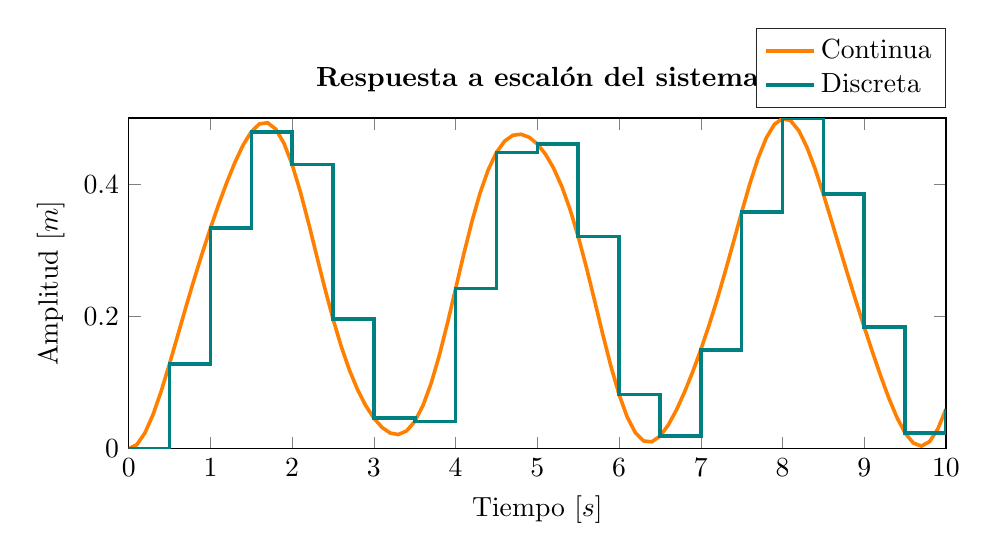
\begin{tikzpicture}

\begin{axis}[%
width=0.856\textwidth,
height=4.2cm,
at={(0\textwidth,0cm)},
scale only axis,
xmin=0,
xmax=10,
xlabel={Tiempo $[s]$},
ylabel={Amplitud $[m]$},
ymin=0,
ymax=0.5,
axis background/.style={fill=white},
title style={font=\bfseries},
title={Respuesta a escalón del sistema},
  legend style={legend cell align=left, at={(1,1.03)}, anchor=south east, align=left, draw=white!15!black}
]
\addplot [color=orange, line width=1.3pt]
  table[row sep=crcr]{%
0	0\\
0.1	0.00619826234325889\\
0.2	0.0241884966128959\\
0.3	0.0522744645694972\\
0.4	0.0879918516868218\\
0.5	0.128559397125211\\
0.6	0.171348848164541\\
0.7	0.214262595367865\\
0.8	0.255933514362603\\
0.9	0.295708674697209\\
1	0.333435041944134\\
1.1	0.369116590796789\\
1.2	0.40254520460955\\
1.3	0.433013918038328\\
1.4	0.459198901192667\\
1.5	0.479251802267866\\
1.6	0.491088190751104\\
1.7	0.492805262748467\\
1.8	0.483126241326124\\
1.9	0.461759279311097\\
2	0.429577721373518\\
2.1	0.388571535598816\\
2.2	0.341575686778064\\
2.3	0.291835961049784\\
2.4	0.24251233507586\\
2.5	0.196234351772937\\
2.6	0.154808500304868\\
2.7	0.119138049010463\\
2.8	0.0893612997287757\\
2.9	0.0651587775916764\\
3	0.0461376271926136\\
3.1	0.0321832351794349\\
3.2	0.0236784574965268\\
3.3	0.0215270687996326\\
3.4	0.0269708009904172\\
3.5	0.0412449869671728\\
3.6	0.0651620147162267\\
3.7	0.0987330986598309\\
3.8	0.140931726432046\\
3.9	0.18966826955869\\
4	0.241993239184747\\
4.1	0.29448976503278\\
4.2	0.343768589085764\\
4.3	0.386953262165954\\
4.4	0.422045844758415\\
4.5	0.448093569811562\\
4.6	0.465126917730837\\
4.7	0.473896614898026\\
4.8	0.475486637810117\\
4.9	0.470909761828616\\
5	0.460794079129878\\
5.1	0.445242840210953\\
5.2	0.423902730337051\\
5.3	0.396219485914543\\
5.4	0.361809089997137\\
5.5	0.320840740630931\\
5.6	0.274322661629965\\
5.7	0.224205015430284\\
5.8	0.173259806542692\\
5.9	0.124754090782935\\
6	0.0819856031791503\\
6.1	0.0477855680938741\\
6.2	0.0241028114268774\\
6.3	0.0117639240594923\\
6.4	0.0104610342321848\\
6.5	0.0189627249935374\\
6.6	0.0354890438981172\\
6.7	0.0581522804825078\\
6.8	0.0853511867475265\\
6.9	0.116021064630686\\
7	0.149681756992704\\
7.1	0.186279805980033\\
7.2	0.225875901158751\\
7.3	0.268270096669663\\
7.4	0.312674472794381\\
7.5	0.357531500275784\\
7.6	0.400539231878859\\
7.7	0.438891099416479\\
7.8	0.46968221403801\\
7.9	0.490390000960276\\
8	0.499316088290222\\
8.1	0.495884040706612\\
8.2	0.480721903439505\\
8.3	0.455510892508611\\
8.4	0.422638623950666\\
8.5	0.384742511429879\\
8.6	0.344254386639084\\
8.7	0.303054600952028\\
8.8	0.26231366056736\\
8.9	0.222549650329354\\
9	0.183873135687835\\
9.1	0.146342435929718\\
9.2	0.110323663155642\\
9.3	0.0767490288518068\\
9.4	0.0471938494651807\\
9.5	0.0237405031690787\\
9.6	0.00865400050690542\\
9.7	0.00394431271297954\\
9.8	0.0109221381171447\\
9.9	0.0298592049657102\\
10	0.0598402724046761\\
};
\addlegendentry{Continua}

\addplot[const plot, color=teal, line width=1.3pt] table[row sep=crcr] {%
0	0\\
0.5	0.128559397125211\\
1	0.333435041944134\\
1.5	0.479251802267865\\
2	0.429577721373517\\
2.5	0.196234351772936\\
3	0.0461376271926133\\
3.5	0.0412449869671727\\
4	0.241993239184747\\
4.5	0.448093569811561\\
5	0.460794079129877\\
5.5	0.32084074063093\\
6	0.0819856031791495\\
6.5	0.0189627249935371\\
7	0.149681756992704\\
7.5	0.357531500275785\\
8	0.499316088290222\\
8.5	0.384742511429878\\
9	0.183873135687834\\
9.5	0.0237405031690781\\
10	0.0598402724046759\\
};
\addlegendentry{Discreta}

\end{axis}
\end{tikzpicture}%

  \caption{Gráfica insertada}
  \label{fig:grafica}
\end{figure}
